\section{Supplementary Materials}
\setcounter{figure}{0}
\begin{figure}[!ht]
\centering
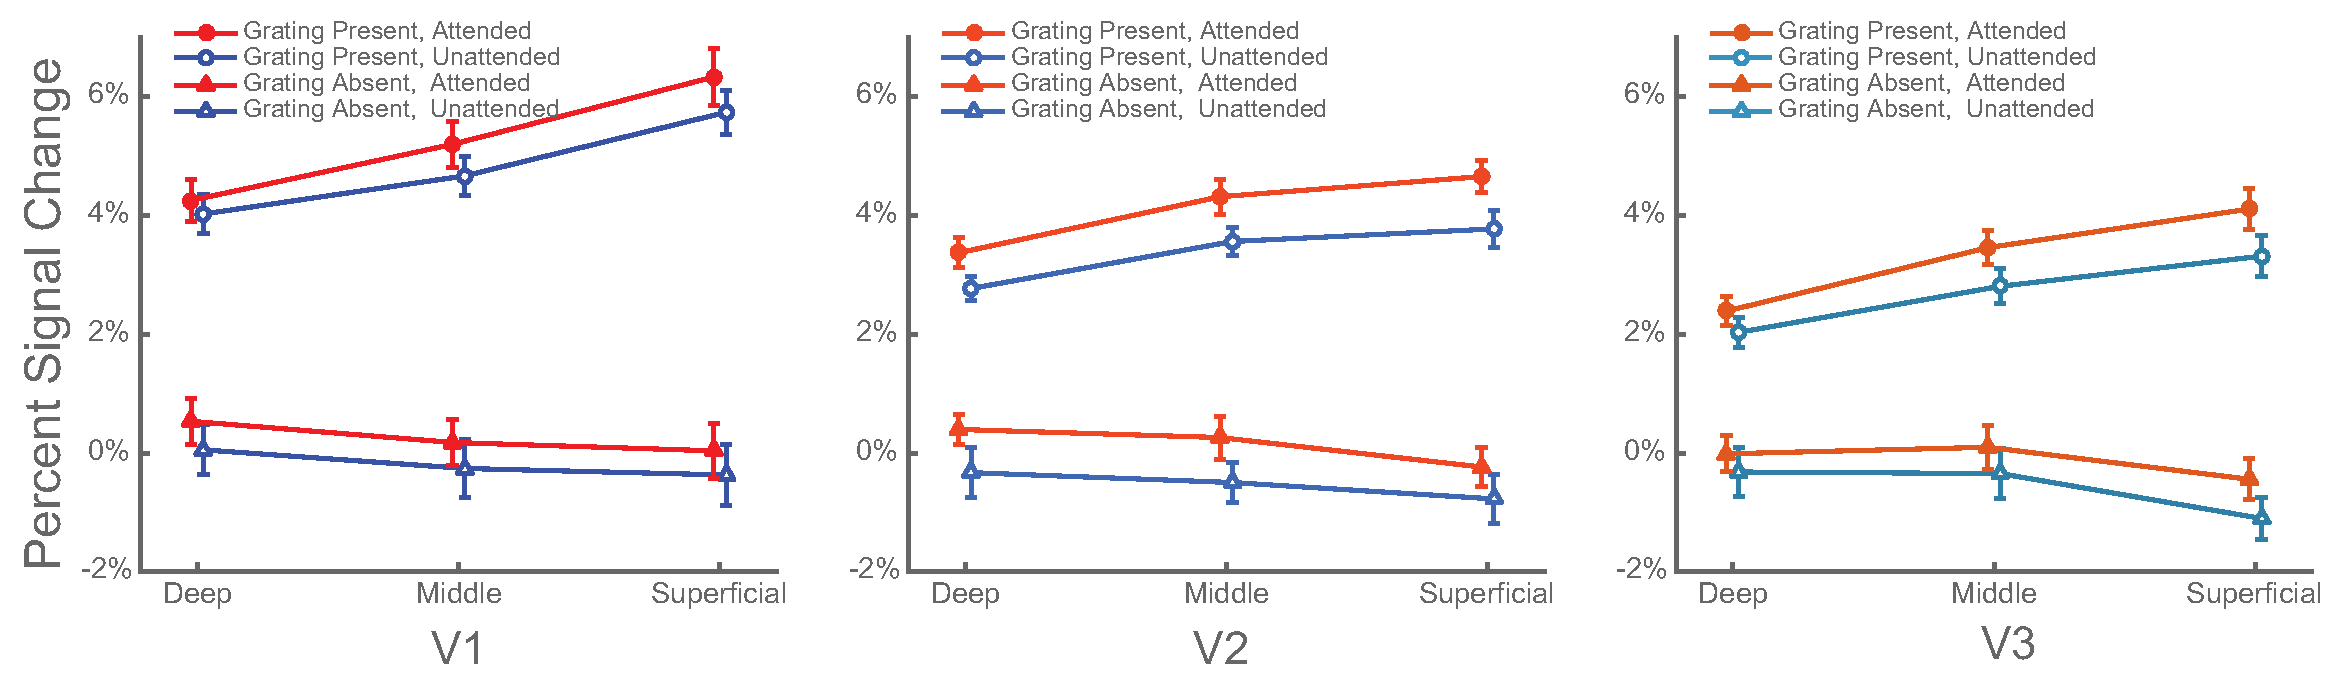
\includegraphics[width=1.0\textwidth, clip=true]{./Chapters/04_Attention/Images/SM_LayerResults_300vertices}
\caption{Control analysis of an ROI with the 300 highest activated vertices.}
\label{fig:layerresults300}
\end{figure}
\begin{figure}[!ht]
\centering
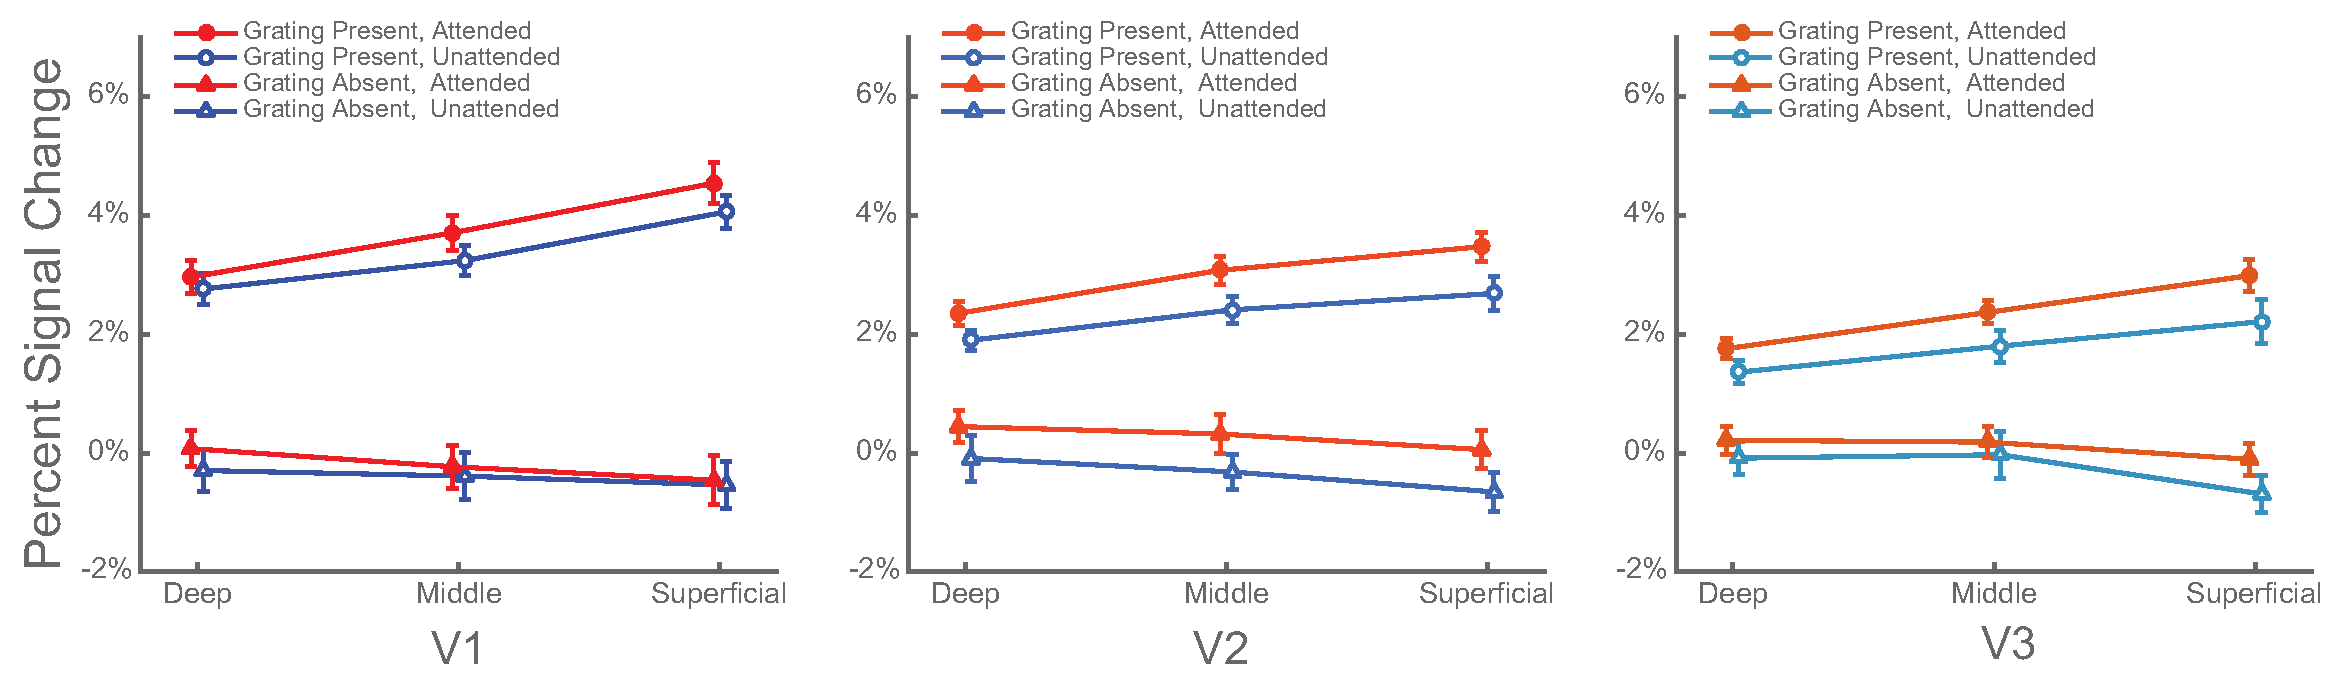
\includegraphics[width=1.0\textwidth, clip=true]{./Chapters/04_Attention/Images/SM_LayerResults_900vertices}
\caption{Control analysis of an ROI with the 900 highest activated vertices.}
\label{fig:layerresults900}
\end{figure}
\begin{figure}[!ht]
\centering
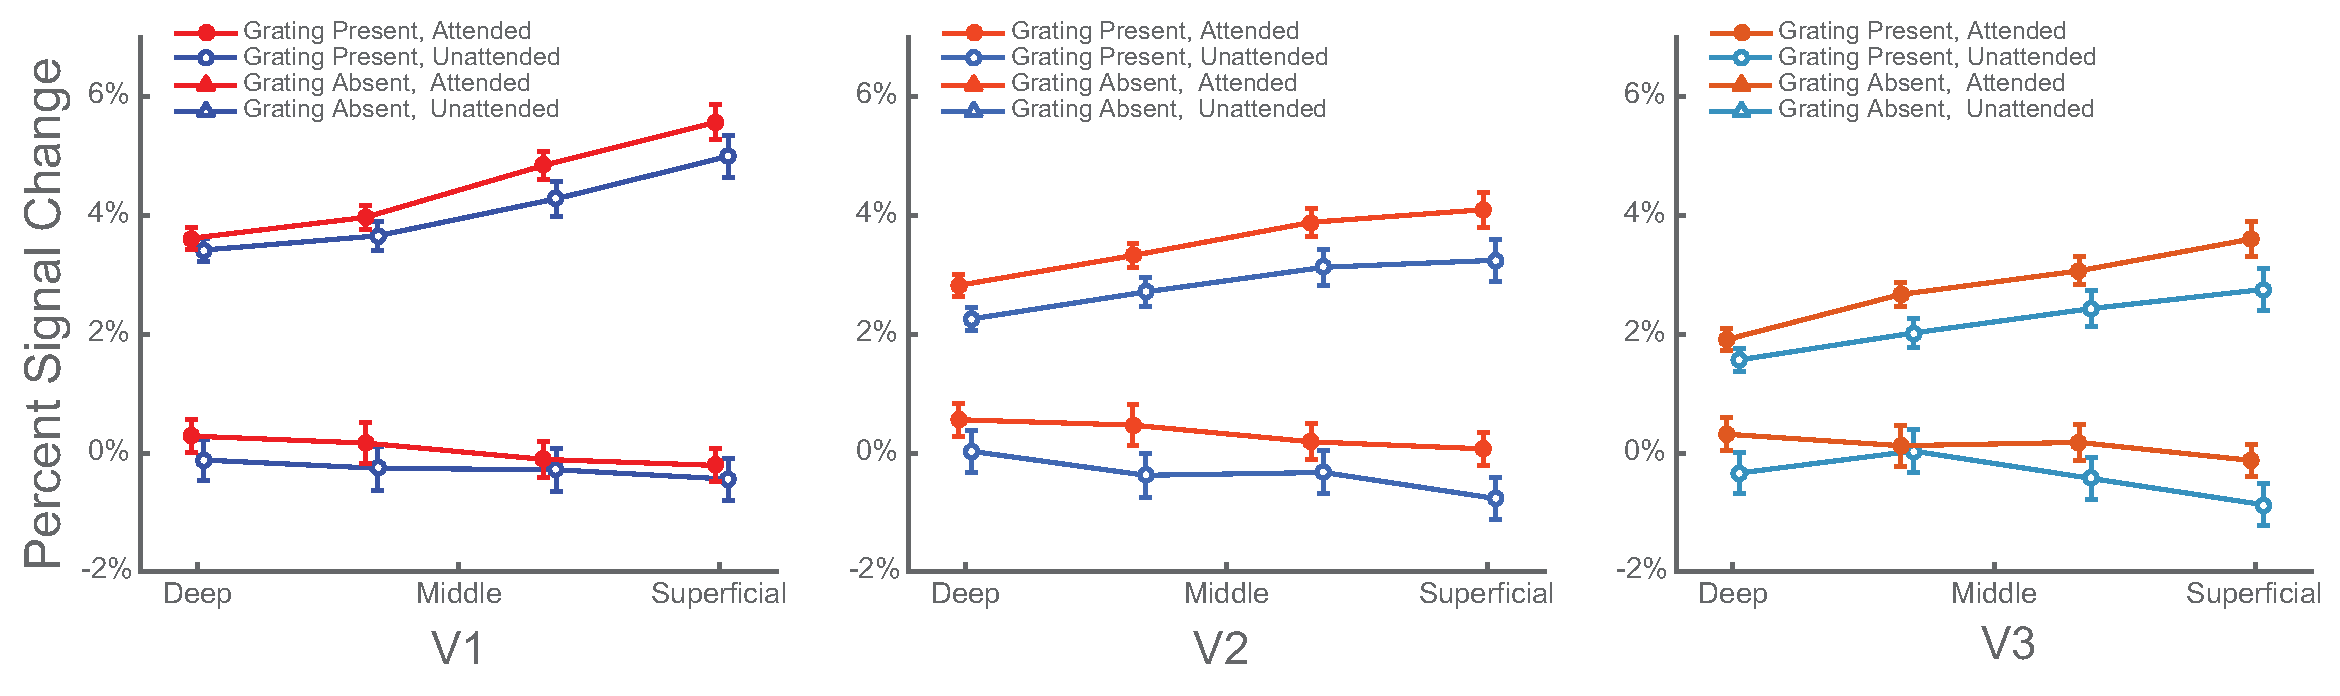
\includegraphics[width=1.0\textwidth, clip=true]{./Chapters/04_Attention/Images/SM_LayerResults_4Layers}
\caption{Control analysis of an ROI with the 600 highest activated vertices, within each of 4 layers.}
\label{fig:layerresults4layers}
\end{figure}
\begin{figure}[!ht]
\centering
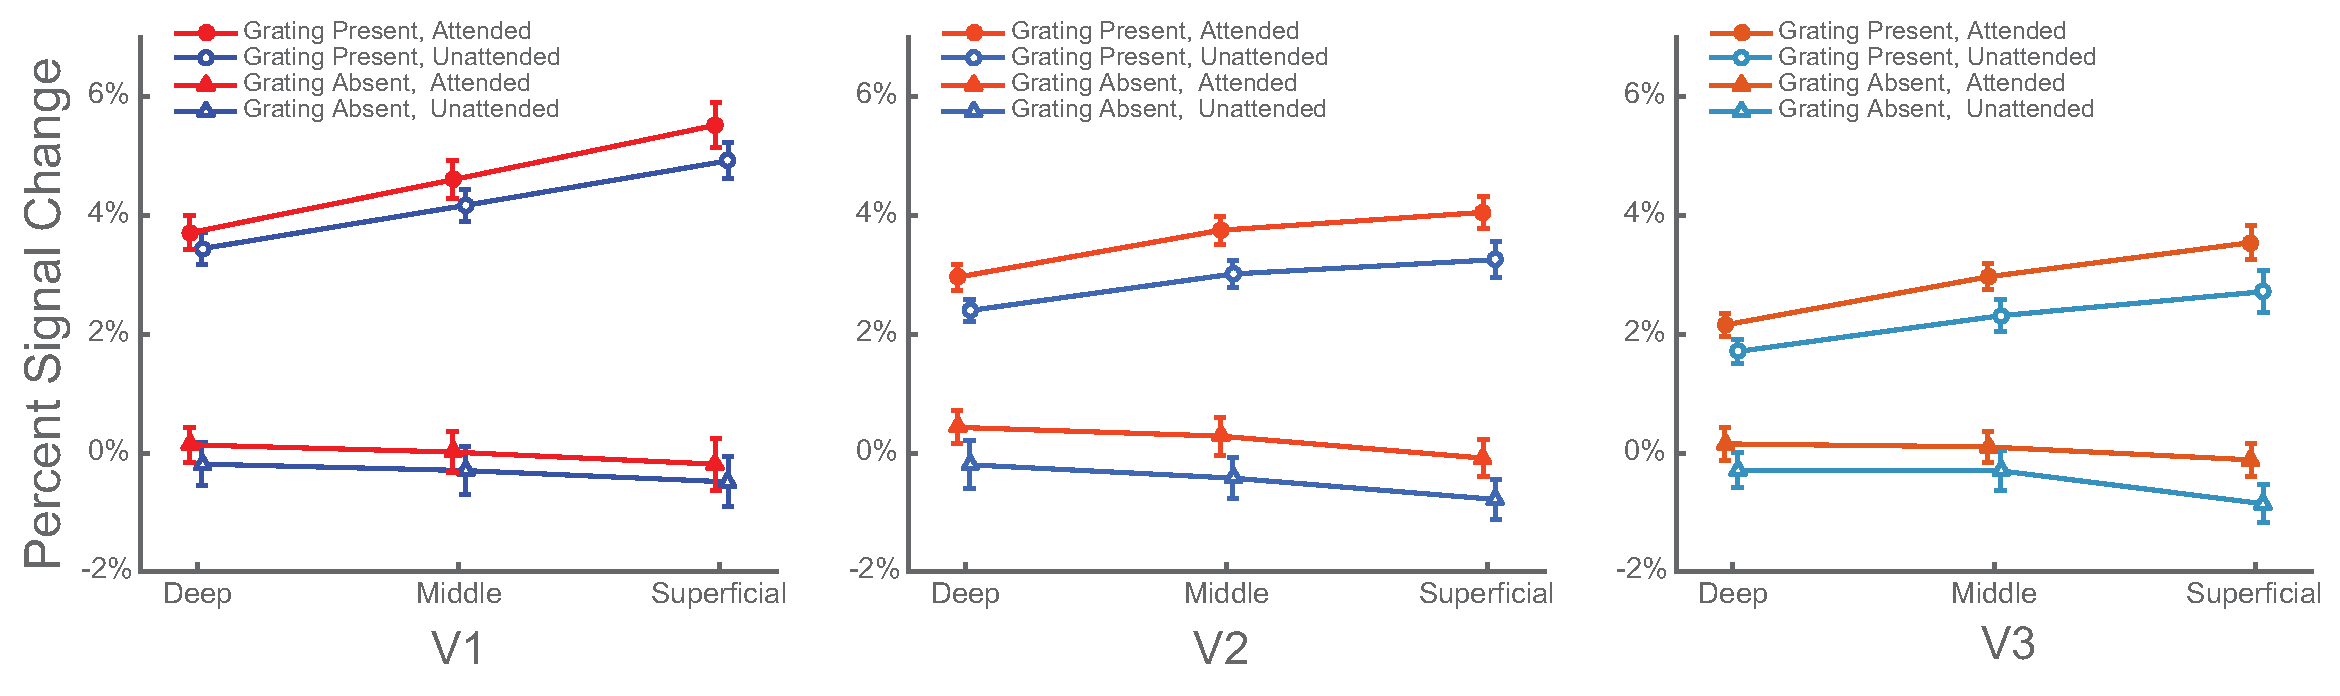
\includegraphics[width=1.0\textwidth, clip=true]{./Chapters/04_Attention/Images/SM_LayerResults_interpolation}
\caption{Control analysis of an ROI with the 600 vertices highest activated vertices, where the laminar signal was obtained by means of interpolation instead of a laminar spatial GLM.}
\label{fig:layerresultsinterp}
\end{figure}
\begin{figure}[!ht]
\centering
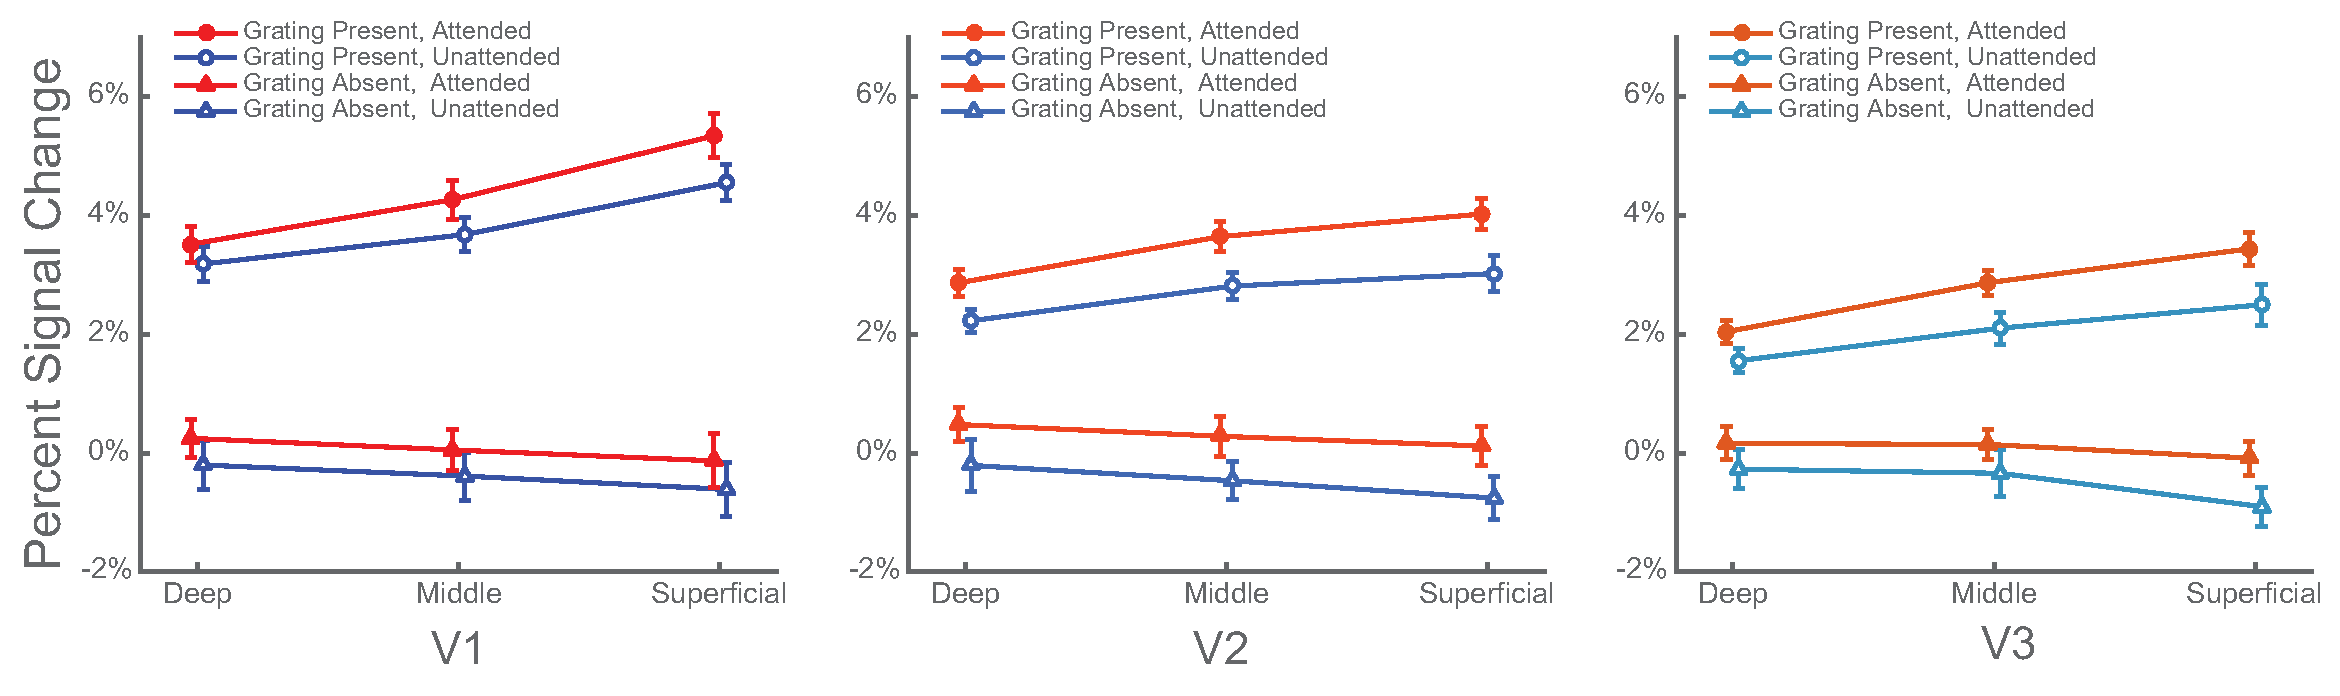
\includegraphics[width=1.0\textwidth, clip=true]{./Chapters/04_Attention/Images/SM_LayerResults_plusAttention}
\caption{Control analysis of an ROI with the 600 vertices highest activated vertices, where the signal from the anticipation window was added to the signal from the stimulus window.}
\label{fig:layerresultsplusattention}
\end{figure}
Figure S1-5. Layer-specific amplitude of the BOLD response in areas V1-V3. Figures S1 and S2 show stimulus and attention-based effects across layers after selecting, respectively, the 300 and 900 most activated vertices (cf. Fig.~\ref{fig:layerresults} in the main text). Figure S3 shows results after defining four cortical layers, rather than three, and Figure S4 depicts results obtained from interpolation instead of a laminar spatial GLM. Error bars indicate $\pm$1 SEM. For figure S5, the signal from the anticipation window was added to the signal from the stimulus window. In all Figures, presenting a stimulus (circles) resulted in a reliable increase in BOLD response from deep to superficial layers. The BOLD response was significantly enhanced for attended locations (red) compared to unattended location (blue) across layers, both when a stimulus was presented and in the absence of visual stimulation. There were only two instances where significance changed compared to the layer analyses that are presented in the main text. The Attention by Layer interaction was not significant in the main analysis (p = 0.114), but was significant in the control analysis when interpolation was used (p = 1.50$\cdot10^{-4}$) and when the signal from the anticipation window was added (p = 0.019). While the Stimulus by Layer by Area interaction was significant in the main analysis (p = 0.015), this interaction failed to reach significance after selecting the 900 most activated vertices (p = 0.12), or when repeating the analysis using four (rather than three) layers (p = 0.056). All other reported results are qualitatively similar to the findings in the main text.
\label{SM5}
\begin{figure}[!ht]
\centering
\includegraphics[width=0.6\textwidth, clip=true]{./Chapters/04_Attention/Images/ExampleBrain}
\caption{Example of Regions of interest on the inflated cortical surface for a representative subject. The label contours from top to bottom show dorsal V3, V2, and V1 and ventral V1, V2, and V3, in both hemispheres. The 600 most activated vertices (highlighted) per region where selected for the main analysis, the 300 and 900 vertices for control analyses in order to show that the effects are independent of size of region of interest.}
\label{fig:roifigures}
\end{figure}
%Random Subject19


%300 vertices:
%The T-values in the region of interest ($\mu \pm \sigma$) were for V1 $T=3.414 \pm 0.950$, for V2 $T=2.728 \pm 0.726$ and for V3 $T=2.562 \pm 0.779$.


%900 vertices:
%The T-values in the region of interest ($\mu \pm \sigma$) were for V1 $T=2.637 \pm 0.828$, for V2 $2.002 \pm 0.715$ and for V3 $1.773 \pm 0.716$.



%A visualisation of the workflow is shown in Fig.~\ref{fig:workflow}.
%\input{./Chapters/04_Attention/Chapters/Figures/FigureWorkflow}


